\subsection{Unknown \texorpdfstring{$\sigma$}{sigma}: T-tests}
\label{subsec:T-test}

As we decided in Section 3, when we don't know the population standard deviation, we estimate it. The resulting T-statistic has the form
\begin{align*}
  t =   \frac{\hat{\theta} - \expc{\hat{\theta}}}{s(\hat{\theta})} = \frac{\hat{\theta} - \expc{\hat{\theta}}}{\sqrt{\widehat{\textnormal{Var}(\hat{\theta})}}}
\end{align*}
In the case when the distribution of $\hat{\theta}$ is Normal, the test is based on Student's T-distribution with acceptance and rejection regions according to the direction of $H_A$:
\begin{enumerate}[label=(\alph*)]
  \item For a \textbf{right-tail alternative},
    \begin{equation}
      \begin{cases}
        \textnormal{reject } H_0 &\textnormal{if } t \geq t_{\alpha}\\
        \textnormal{accepts } H_0 &\textnormal{if } t < t_{\alpha}\\
      \end{cases}
    \end{equation}
  
  \item For a \textbf{left-tail alternative},
    \begin{equation}
      \begin{cases}
        \textnormal{reject } H_0 &\textnormal{if } t \leq -t_{\alpha}\\
        \textnormal{accepts } H_0 &\textnormal{if } t > -t_{\alpha}\\
      \end{cases}      
    \end{equation}
  
  \item For a \textbf{two-sided alternative},
    \begin{equation}
      \begin{cases}
        \textnormal{reject } H_0 &\textnormal{if } |t| \geq t_{\alpha/2}\\
        \textnormal{accepts } H_0 &\textnormal{if } |t| < t_{\alpha/2}\\
      \end{cases}
    \end{equation}
\end{enumerate}
Quantiles $t_{\alpha}$ and $t_{\alpha/2}$ are given in Table A5 (in textbook). As in Section 3.4, the number of degrees of freedom depends on the problem and the sample size, see Table 2 and formula (10)
\end{multicols}

\begin{figure}[H]
  \centering
  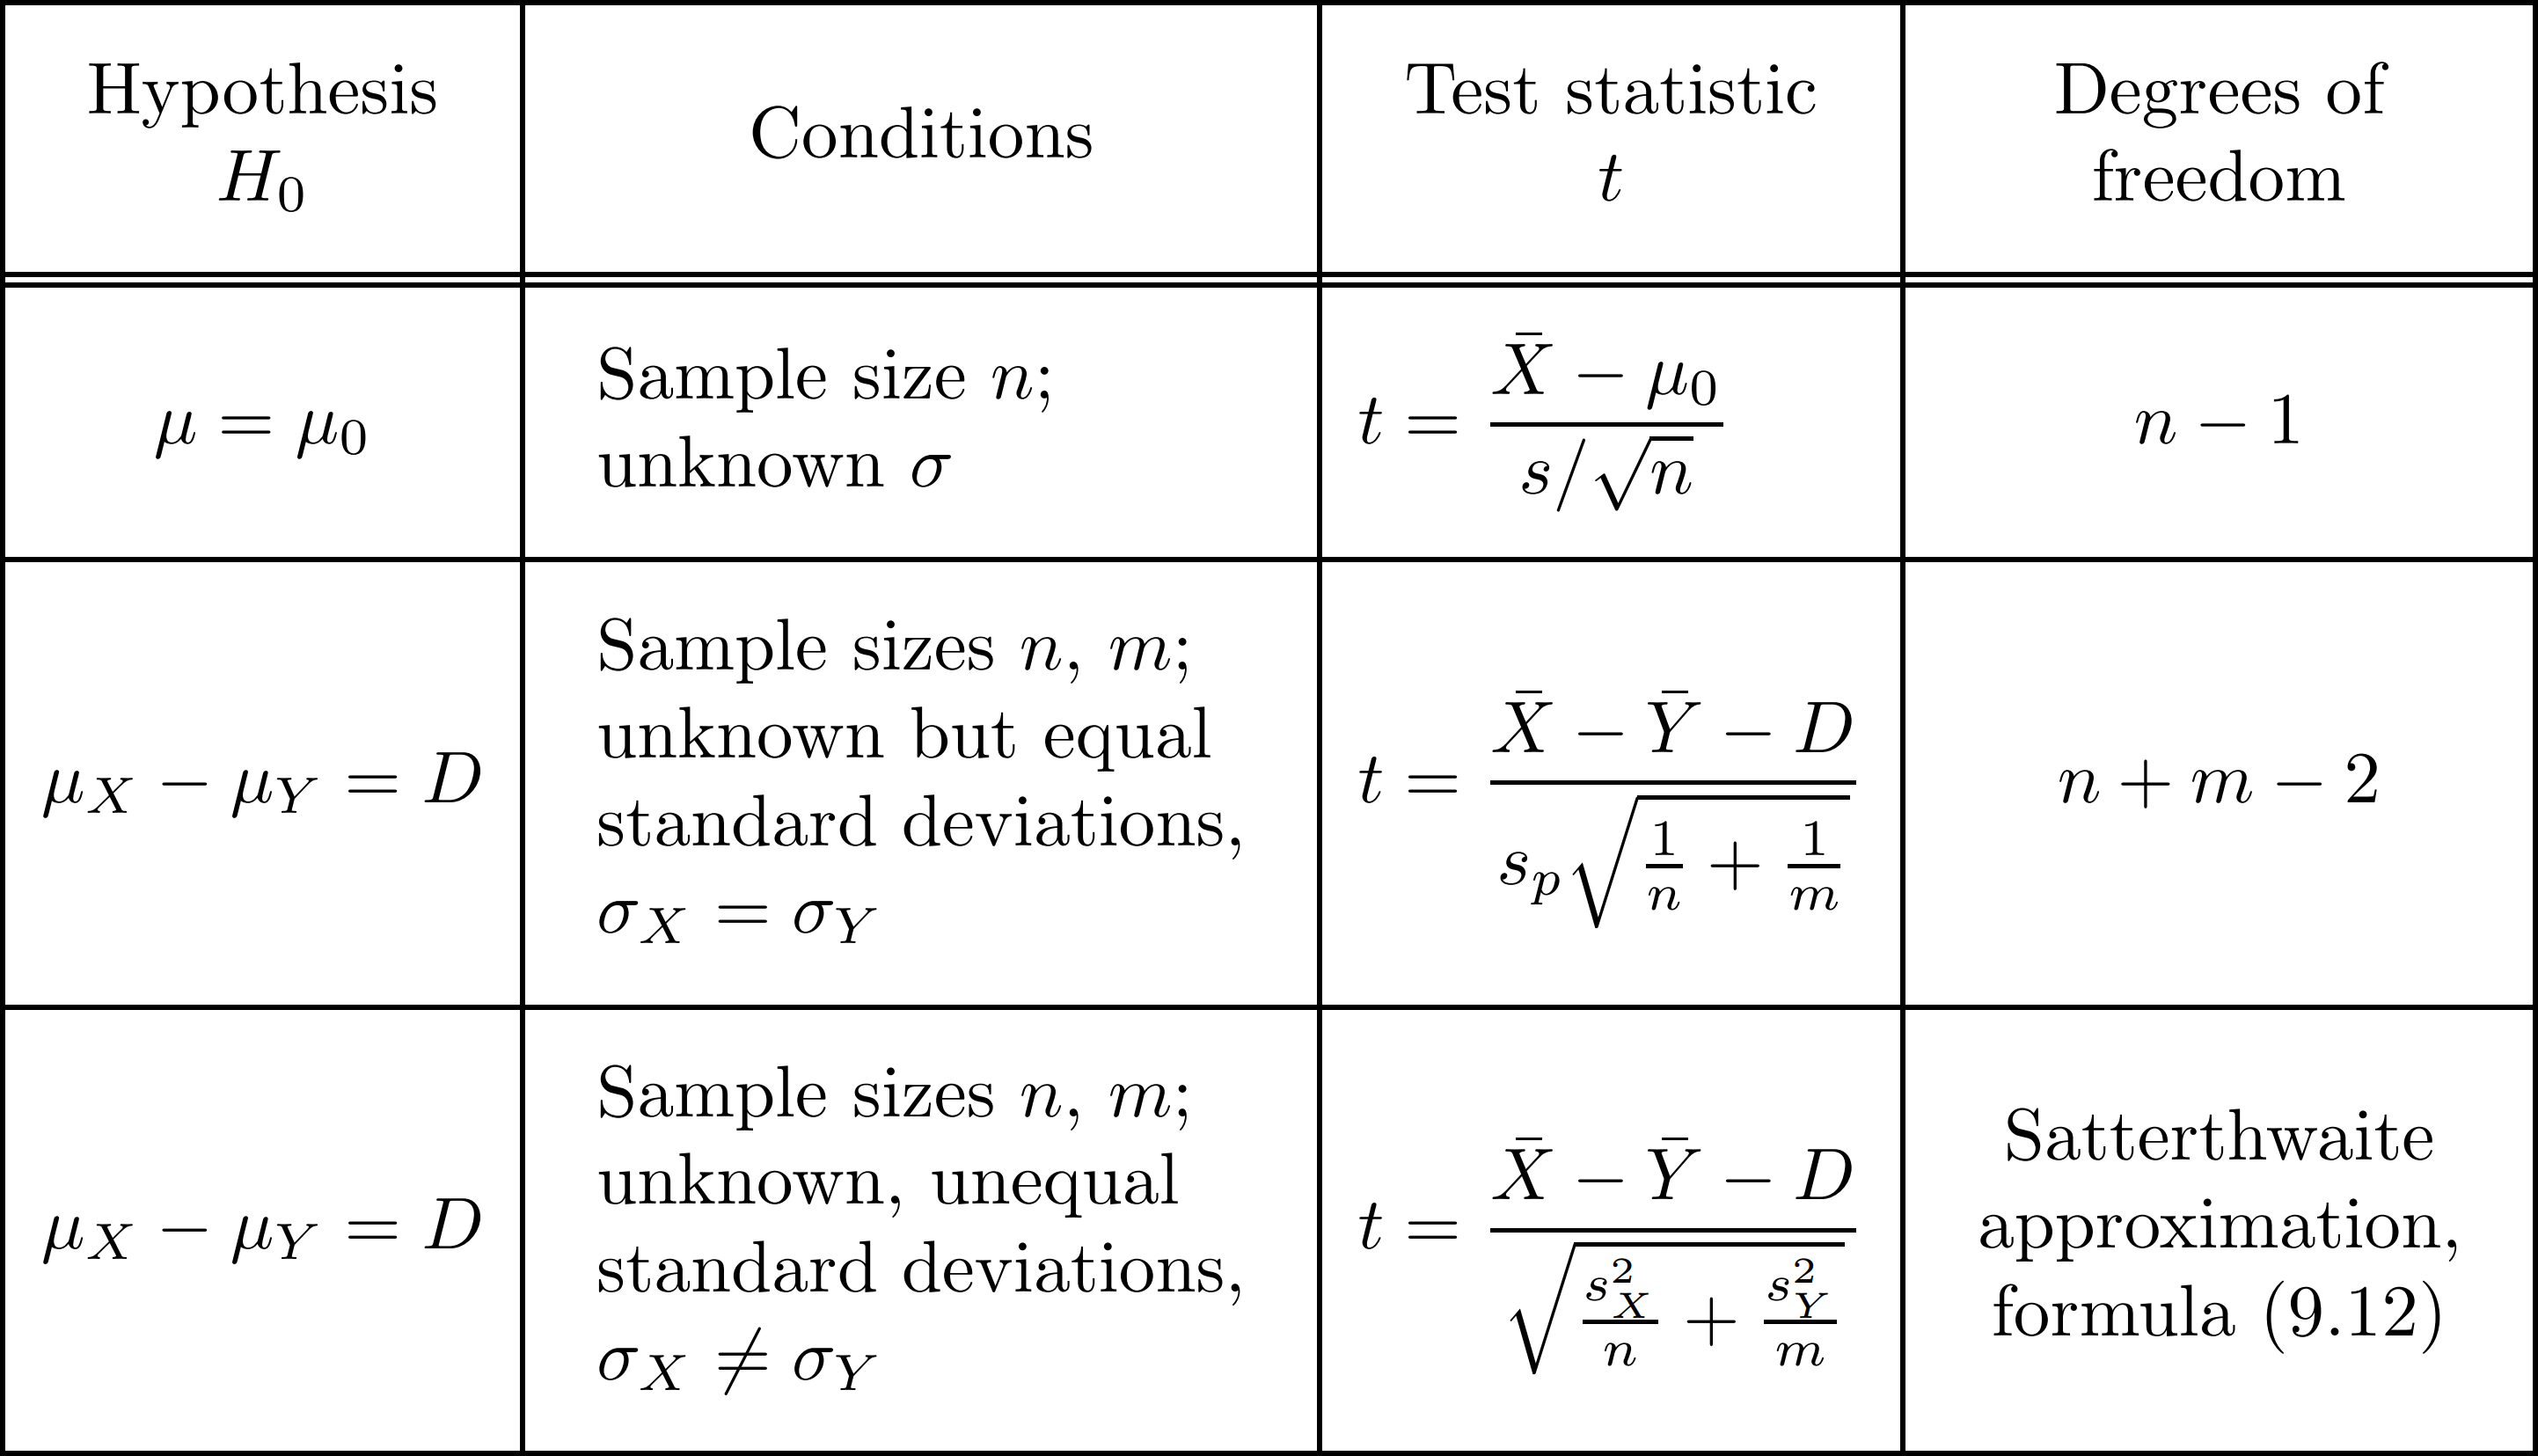
\includegraphics[width=\linewidth]{img/table-9.2.png}
  \caption*{\textbf{Table 2:} \textit{Summary of T-tests}}
  \label{table2}
\end{figure}

\begin{multicols}{2}
\setlength{\columnsep}{1.5cm}
\setlength{\columnseprule}{0.2pt}

As in Section 3.4, the \textbf{pooled sample variance}
\begin{align*}
  s_p^2 &= \frac{\dsum_{i = 1}^{n} (X_i - \bar{X})^2 + \dsum_{i = 1}^{m} (Y_i - \bar{Y})^2}{n + m - 2} \\
  &= \frac{(n - 1) s_X^2 + (m - 1) s_Y^2}{n + m - 2}
\end{align*}
is computed for the case of equal unknown variances. When variances are not equal, degrees of freedom are computed by Satterthwaite approximation (12).

\textbf{\textit{Check examples 9.28, 9.29, 9.30 in the textbook}}.

When the distribution of $\hat{\theta}$ is not Normal, the Student's \textit{T-distribution} cannot be used. The distribution of a T-statistic and all its probabilities will be different from Student's T, and as a result, our test may not have the desired significance level.
